\begin{figure}[H]
\centering
\begin{minipage}[b]{0.49\textwidth}
\centering
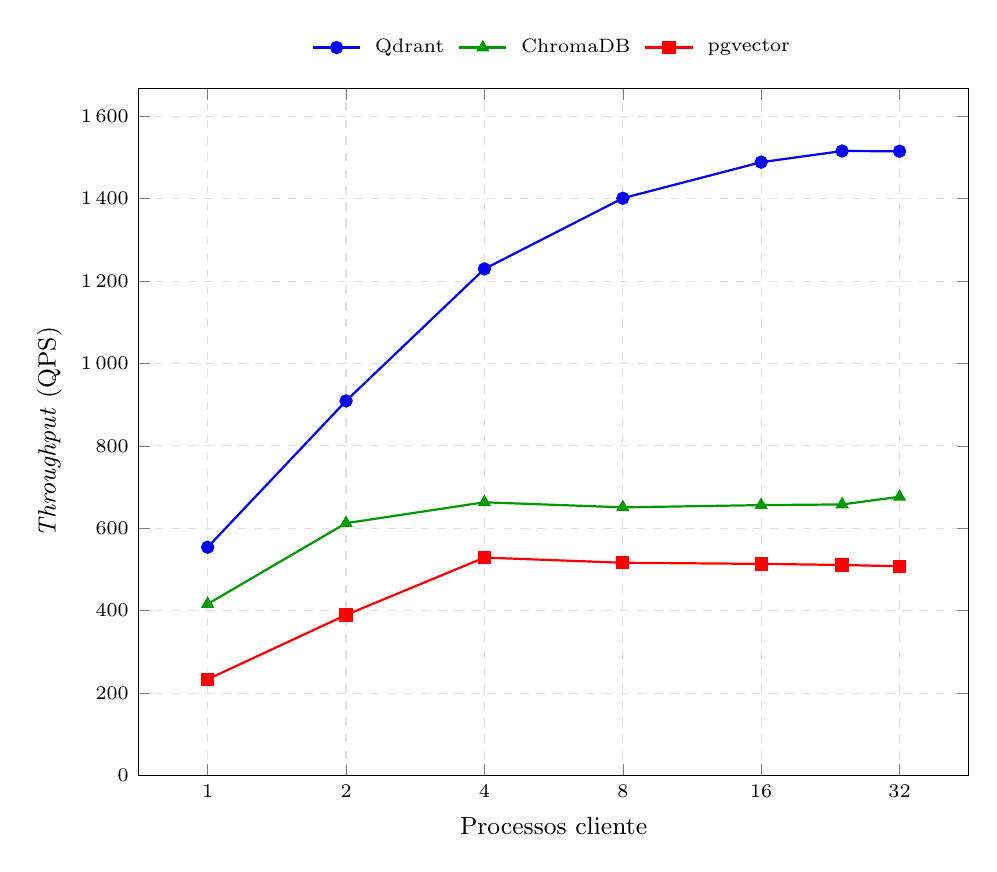
\begin{tikzpicture}
\begin{axis}[
    width=\textwidth, height=0.85\textwidth,
    xlabel={Processos cliente}, ylabel={\textit{Throughput} (QPS)},
    xmode=log, log basis x={2}, xtick={1,2,4,8,16,32}, xticklabels={1,2,4,8,16,32},
    ymin=0,
    /pgf/number format/1000 sep={\,},
    grid=major, grid style={dashed, gray!25},
    legend columns=3, legend style={at={(0.5,1.03)}, anchor=south, font=\scriptsize, draw=none, /tikz/column sep=3pt},
    tick label style={font=\scriptsize}, label style={font=\small}
]
\addplot[color=blue, mark=*, thick] coordinates {(1,554.15) (2,909.21) (4,1229.52) (8,1401.05) (16,1488.53) (24,1515.59) (32,1515.03)};
\addlegendentry{Qdrant}
\addplot[color=green!60!black, mark=triangle*, thick] coordinates {(1,416.38) (2,612.54) (4,663.21) (8,650.93) (16,656.32) (24,658.00) (32,676.57)};
\addlegendentry{ChromaDB}
\addplot[color=red, mark=square*, thick] coordinates {(1,233.74) (2,389.79) (4,529.07) (8,516.45) (16,513.74) (24,511.12) (32,507.87)};
\addlegendentry{pgvector}
\end{axis}
\end{tikzpicture}
\caption*{(a) \textit{Throughput}}
\end{minipage}%
\hfill
\begin{minipage}[b]{0.49\textwidth}
\centering
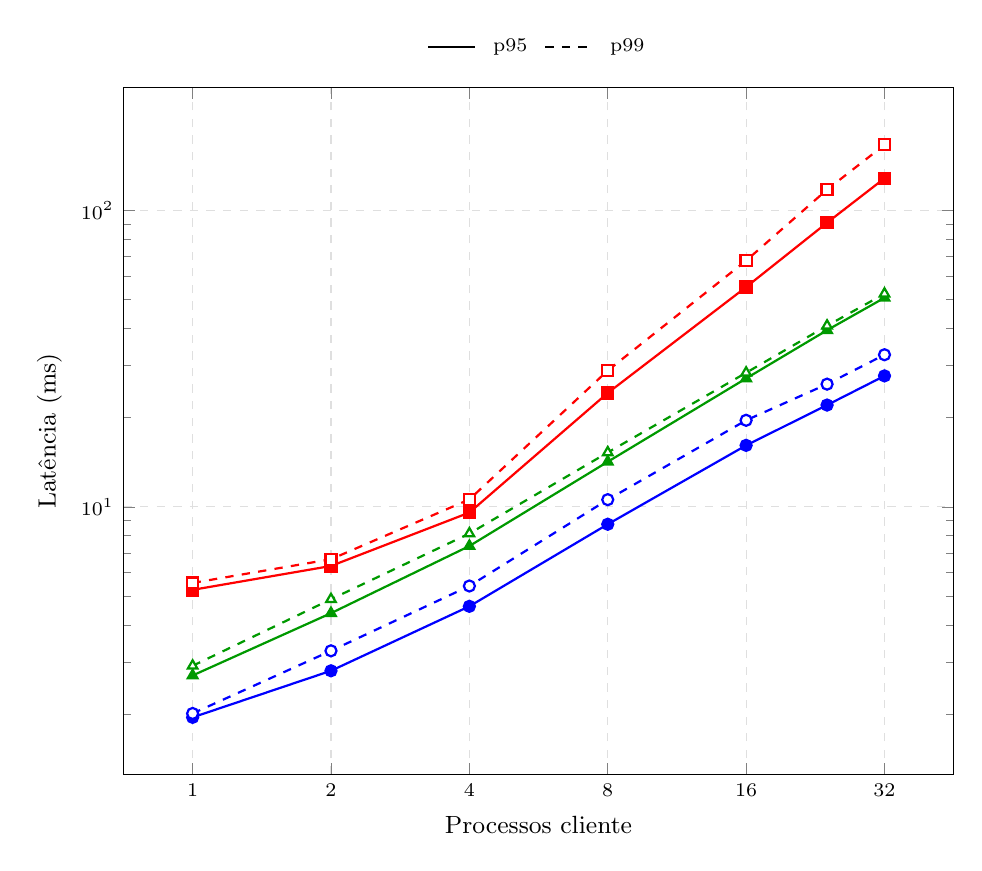
\begin{tikzpicture}
\begin{axis}[
    width=\textwidth, height=0.85\textwidth,
    xlabel={Processos cliente}, ylabel={Latência (ms)},
    xmode=log, log basis x={2}, xtick={1,2,4,8,16,32}, xticklabels={1,2,4,8,16,32},
    ymode=log, log basis y={10},
    /pgf/number format/1000 sep={\,},
    grid=major, grid style={dashed, gray!25},
    legend columns=2, legend style={at={(0.5,1.03)}, anchor=south, font=\scriptsize, draw=none, /tikz/column sep=4pt},
    tick label style={font=\scriptsize}, label style={font=\small}
]
\addplot[color=blue, mark=*, thick, forget plot] coordinates {(1,1.95) (2,2.80) (4,4.62) (8,8.74) (16,16.13) (24,22.06) (32,27.67)};
\addplot[color=blue, mark=*, mark options={solid, fill=white}, thick, dashed, forget plot] coordinates {(1,2.01) (2,3.27) (4,5.41) (8,10.58) (16,19.60) (24,25.95) (32,32.61)};
\addplot[color=green!60!black, mark=triangle*, thick, forget plot] coordinates {(1,2.70) (2,4.38) (4,7.38) (8,14.20) (16,27.13) (24,39.46) (32,50.75)};
\addplot[color=green!60!black, mark=triangle*, mark options={solid, fill=white}, thick, dashed, forget plot] coordinates {(1,2.91) (2,4.88) (4,8.13) (8,15.26) (16,28.35) (24,40.84) (32,52.36)};
\addplot[color=red, mark=square*, thick, forget plot] coordinates {(1,5.25) (2,6.32) (4,9.57) (8,24.23) (16,55.16) (24,90.94) (32,128.40)};
\addplot[color=red, mark=square*, mark options={solid, fill=white}, thick, dashed, forget plot] coordinates {(1,5.54) (2,6.66) (4,10.60) (8,28.84) (16,67.74) (24,117.59) (32,166.50)};
\addlegendimage{black, thick}\addlegendentry{p95}
\addlegendimage{black, thick, dashed}\addlegendentry{p99}
\end{axis}
\end{tikzpicture}
\caption*{(b) Latências p95 e p99}
\end{minipage}
\caption{\textit{Throughput} e latências p95 e p99 sob concorrência crescente para a \textbf{Similaridade de Cosseno} (mediana de 3 réplicas). No painel (b), cada motor mantém a cor do painel (a); a linha contínua corresponde ao p95 e a tracejada ao p99, em escala logarítmica.}
\label{fig:throughput_concorrencia_cosine}
\end{figure}
